%%%%%% DON'T MODIFY STARTING HERE
\section*{1. Fundamentals}

In this course, you will work with a tabletop robot arm called the \textbf{\href{https://www.wlkata.com/products/wlkata-mirobot-introduction}{Mirobot}}.
This first exercise will help you learn the fundamentals of using this robot.

\paragraph{1A.} Robot Use Agreement. Read carefully the Do's and Don'ts with handling the robot on this \href{https://forms.gle/hHMYKivbUgeGQurR7}{Google Form} and submit the form.
Once done, please attach a screenshot of your submission in the space provided.

\danger~\textbf{\underline{Note}}: You will need to fill out this form \textbf{every single time} you use the robot.


\paragraph{1B.} Install the latest version of the WLKATA Studio software \href{https://www.wlkata.com/support/download-center }{here}. For Windows users, additionally install the driver (more instructions can be found \href{https://document.wlkata.com/?doc=/wlkata-mirobot-user-manual/12-quick-start-guide-of-mirobot/#header-three-el91d}{here}.)
Once done, please attach a screenshot of the WLKATA Studio software running on your computer in the space provided.

\paragraph{1C.} Set up hardware: plug in the USB cable and power on the robot by pressing the on/off button on the base of robot, as shown in the image below.
Please attach a photo of the robot switched on in the space provided.

\begin{figure}[H]
  \centering
  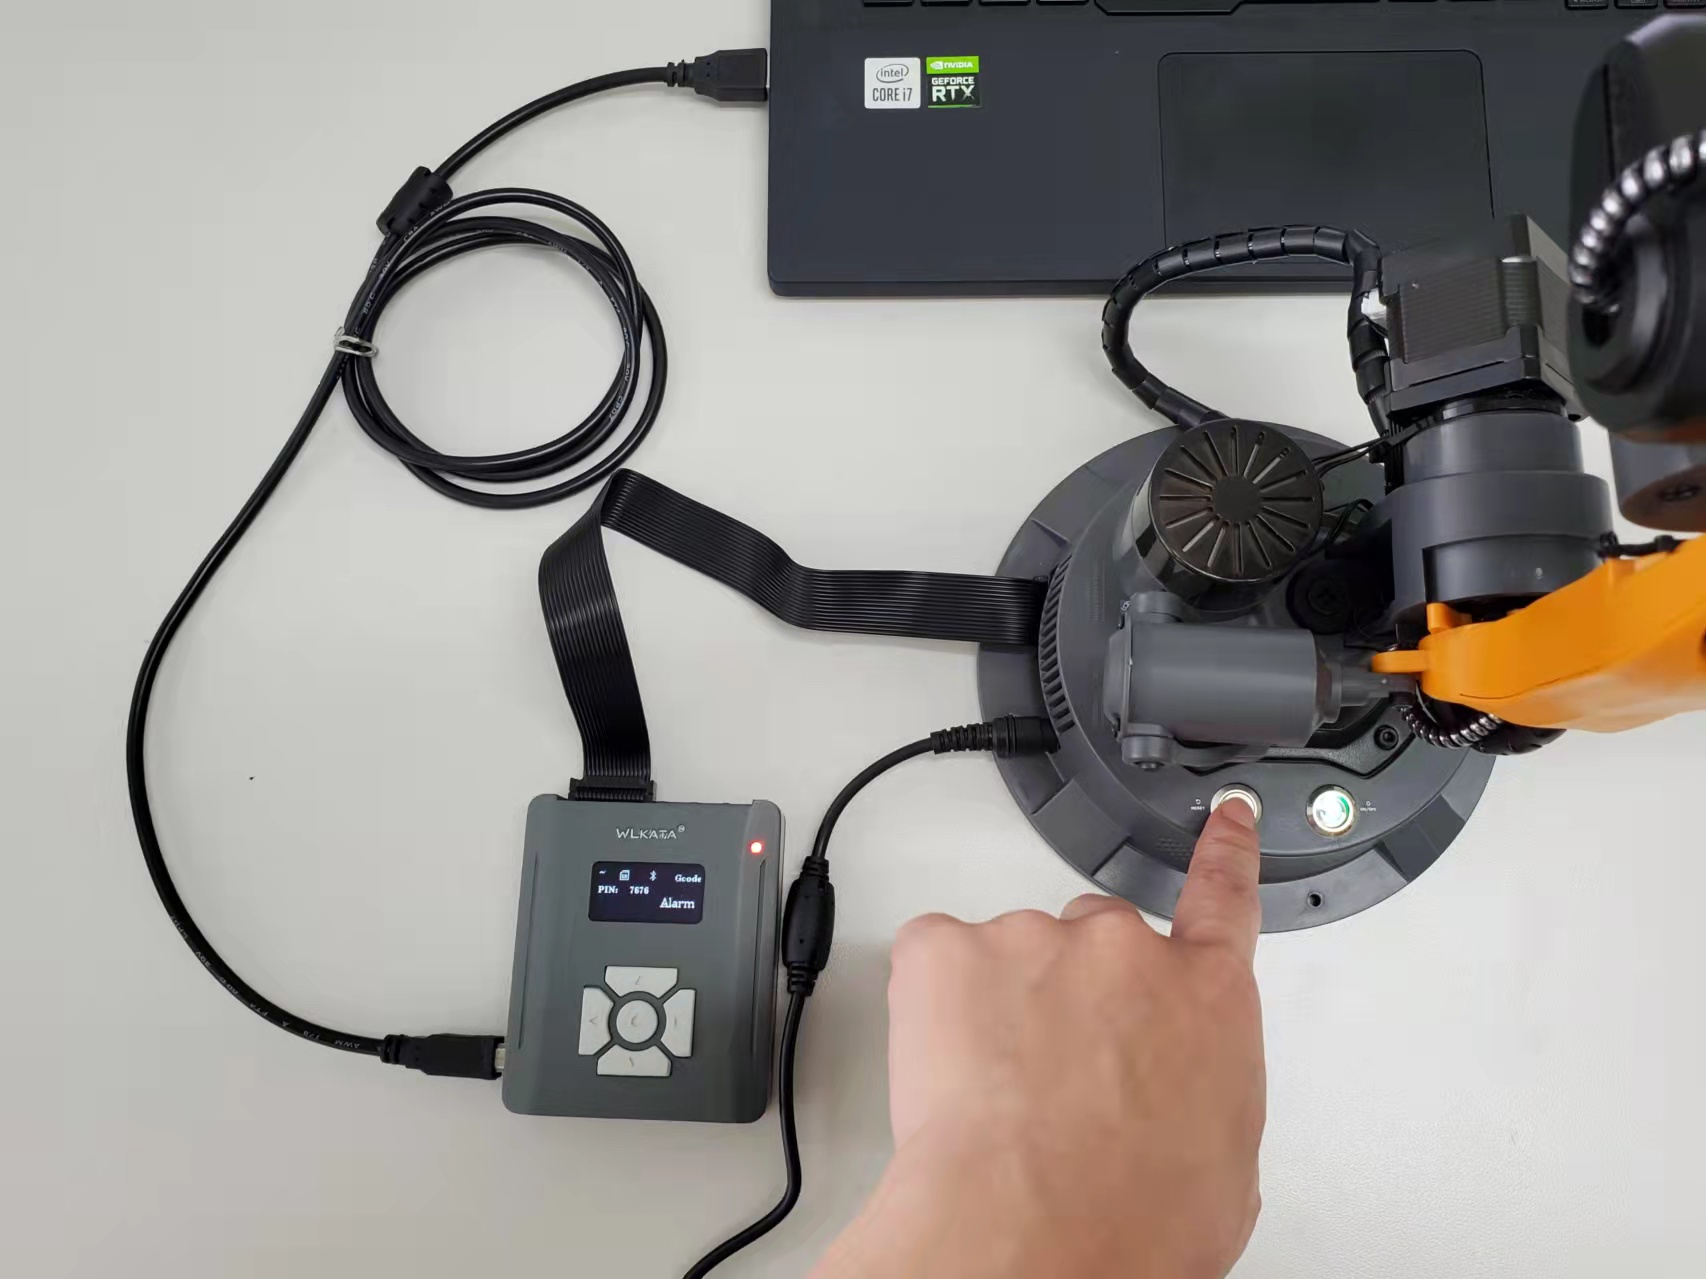
\includegraphics[width=10cm]{image/hardware_setup.jpg}
  \caption*{Powering on the Mirobot. The power button is to the right of the one the person above is pressing.}
%   \label{fig:galaxy}
\end{figure}

\paragraph{1D.} Check connection.
\begin{enumerate} %[(i)]
    \item Open WLKATA Studio.
    \item If the upper left corner of the WLKATA Studio interface displays CONNECTED, you are successfully connected. Otherwise, you may need to change the COM setting (\href{https://document.wlkata.com/?doc=/wlkata-mirobot-user-manual/12-quick-start-guide-of-mirobot/#header-three-6hmdl}{more details}).
    \item  When the robotic arm is powered on, or when the serial port connection is first established, each axis of the robotic arm is locked. To unlock the axes and perform any operations, the robotic must be homed. Click the HOMING button in the WLKATA Studio. Wait for the manipulator to be homed. Please attach a photo of your robot after the homing operation. It should look like the one below.
\end{enumerate}
\begin{figure}[H]
  \centering
  \vspace*{-0.0 in}
  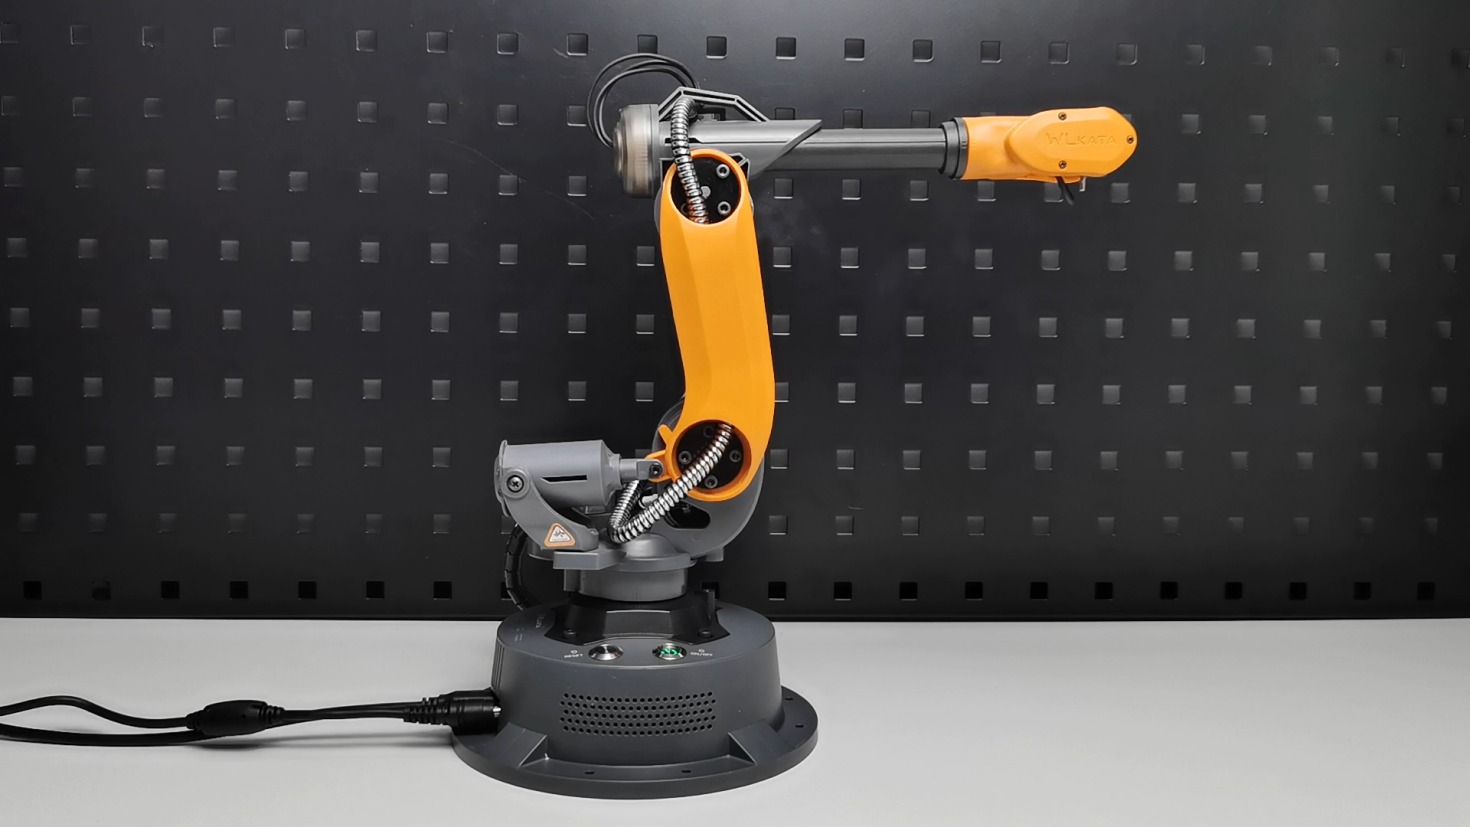
\includegraphics[width=10cm]{image/post_homing.png}
  \caption*{The correct position of the manipulator after a successful HOMING action}
%   \label{fig:galaxy}
\end{figure}


\paragraph{1E.} Inverse Kinematics.\\
\noindent Set the robot mode to \textbf{COORD MODE} (\href{https://document.wlkata.com/?doc=/wlkata-mirobot-user-manual/12-quick-start-guide-of-mirobot/\#header-three-2mfvd}{more details}) within the studio to move the robot arm to a target position marked \texttt{TARGET A} on the mat.
Submit photo result in the space provided.



\paragraph{1F.} Forward Kinematics.\\
\noindent Set the robot to \textbf{JOINT MODE} (\href{https://document.wlkata.com/?doc=/wlkata-mirobot-user-manual/12-quick-start-guide-of-mirobot/\#header-three-2mfvd}{more details}) within the studio to move the robot arm to a target position marked \texttt{TARGET B} on the mat. Submit photo result in the space provided.
%%%%%% DON'T MODIFY UNTIL HERE

\newpage

\paragraph{Answers.}
Please do not exceed the height provided for each answer image.
%%%%%% YOU ANSWER STARTS HERE

% NOTE: MAKE SURE YOU DON'T CHANGE THE HEIGHT OF IMAGES
% NOTE: MAKE SURE TO REMOVE THE 'draft' OPTION FOR includegraphics BELOW. OTHERWISE, YOU WILL NOT SEE YOUR IMAGES.

\paragraph{1A. Robot Use Agreement}
\begin{center}
    \includegraphics[draft,height=2.5in]{YOUR\_ANSWER.png}
\end{center}

\paragraph{1B. WLKATA Studio}
\begin{center}
    \includegraphics[draft,height=2.5in]{YOUR\_ANSWER.png}
\end{center}

\newpage
\paragraph{1C. Set up hardware}
\begin{center}
    \includegraphics[draft,height=2.5in]{YOUR\_ANSWER.png}
\end{center}

\paragraph{1D. Check Connection}
\begin{center}
    \includegraphics[draft,height=2.5in]{YOUR\_ANSWER.png}
\end{center}

\newpage
\paragraph{1E. Inverse Kinematics}
\begin{center}
    \includegraphics[draft,height=2.5in]{YOUR\_ANSWER.png}
\end{center}

\paragraph{1F. Forward Kinematics}
\begin{center}
    \includegraphics[draft,height=2.5in]{YOUR\_ANSWER.png}
\end{center}

\newpage

\paragraph{Additional Space.}
Please do not exceed this page for this question.
%%%%%% YOU ANSWER ENDS HERE
